%
%  Peter Vermeer
%
\documentclass[12pt,fullpage]{article}
\usepackage{fullpage}
\usepackage{psfrag}                                          % LaTeX graphics tool
\usepackage{pslatex}                                         % avoids the default cmr font
\usepackage{graphicx}                                        % graphics package 
\usepackage{epsfig}                                          % figures
\usepackage{epsfig} 
\usepackage{hyperref}
\usepackage{color}

\begin{document}

\noindent
{\bf Cauchy distribution} (from \color{blue}\url{http://www.math.wm.edu/~leemis/chart/UDR/UDR.html}\color{black})

\noindent
The shorthand $X \sim {\rm Cauchy}(a,\alpha)$ is used to indicate that the
random variable $X$ has the Cauchy distribution with positive scale parameter $\alpha$ and location parameter $a$.
A Cauchy random variable $X$ with parameters $a$ and $\alpha$ has probability density function 
$$
f(x) = \frac{1} {\alpha \kern 0.08 em \pi [1 + ((x - a) / \alpha) ^ 2]} \qquad \qquad -\infty < x < \infty
$$
for $\alpha > 0$ and $-\infty < a < \infty$.
The Cauchy distribution is of interest because its moments are undefined.
The probability density function for various combinations of $a$ and $\alpha$ is given below. 
{\begin{figure}[h!]
\begin{center}
\psfrag{lab1}{$a \kern -0.08 em = \kern -0.08 em  1,\, \alpha \kern -0.08 em  = \kern -0.08 em  0.25$}
\psfrag{lab2}{$a \kern -0.08 em  = \kern -0.08 em  2,\, \alpha \kern -0.08 em  = \kern -0.08 em  0.5$}
\psfrag{lab3}{$a \kern -0.08 em  = \kern -0.08 em  3,\, \alpha \kern -0.08 em  = \kern -0.08 em  1$}
\psfrag{labx}{$x$}
\psfrag{labf}{$f(x)$}
\includegraphics[width=3.2in]{CauchyPlot.ps}
\end{center}
\end{figure}}\\
The cumulative distribution function on
the support of $X$ is
$$
F(x) = P(X \le x) = \frac{1} {2 \kern 0.08 em \pi} \, \left( \pi - 2 \,\arctan \left( {\frac {a - x} {{\alpha}}} \right)  \right) \qquad \qquad -\infty < x < \infty.
$$
The survivor function on the support of $X$ is
$$
S(x) = P(X \ge x) = \frac{1} {2 \kern 0.08 em \pi} \, \left( \pi + 2 \,\arctan \left( {\frac {a - x} {{\alpha}}} \right)  \right) \qquad \qquad -\infty < x < \infty.
$$
The hazard function on the support of $X$ is
$$
h(x) = \frac{f(x)} {S(x)} = 2 \,\alpha  \left( {\alpha } ^ {2} - 2 \, x a + {a} ^ {2} + {x} ^ {2} \right) ^ {-1} \left( \pi + 2 \, \arctan \left( {\frac {a - x} {\alpha }} \right)  \right) ^ {\kern -0.08 em -1} \qquad \qquad -\infty < x < \infty.
$$
The cumulative hazard function on the support of $X$ is
$$
H(x) = - \ln S(x) = \ln  \left( 2 \pi \right) - \ln  \left( \pi  + 2 \, \arctan \left( {\frac {a - x} {\alpha }} \right)  \right)  \qquad \qquad -\infty < x < \infty.
$$
The inverse distribution function of $X$ is
$$
F ^ {-1}(u) = a - \alpha \cot \left( \pi \kern 0.08 em u \right) \qquad \qquad 0 < u < 1.
$$
The population median of $X$ is the location parameter, $a$.\\
\\
\noindent
The population moments of $X$ are undefined. It follows that the population mean, variance, skewness, and kurtosis of $X$ are also undefined.

\vspace{0.1in}
\noindent
{\bf APPL verification:}
The APPL statements
\begin{verbatim}
X := CauchyRV(a, alpha);
CDF(X);
SF(X);
HF(X);
IDF(X);
Mean(X);
Variance(X);
Skewness(X);
Kurtosis(X);
MGF(X);
\end{verbatim}
verify the cumulative distribution function, survivor function, hazard function, mean, variance, skewness, kurtosis, and moment generating function.
\end{document}
